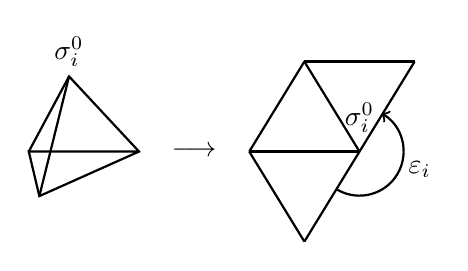
\begin{tikzpicture}[scale=1]
 \def\a{1.40}
 \def\b{0.5}
 \def\trigConst{0.816497}

 \begin{scope} [x     = {(1cm,0)},
   y     = {({0.7cm*cos(135)},{-0.7cm*sin(135)})},
   z     = {(0,1cm)}]


  \path coordinate (T1) at ({-(0.5*\a)}, {0.3333*\trigConst*\a}, {\trigConst*\a})
  coordinate (A1) at (0,0,0)
  coordinate (B1) at ({-\a},0,0)
  coordinate (C1) at ({-(0.5*\a)},{\trigConst*\a},0)
  coordinate (E1) at ({-(0.5*\a)}, {0.3333*\trigConst*\a}, {-\trigConst*\a});

  \draw[thick]  (A1) -- (B1) -- (C1) -- (A1) -- (T1) -- (B1);
  \draw[thick]  (T1) -- (C1);
  \node(h1)[anchor=south] at (T1) {$\sigma^0_i$};

 \end{scope}
 \node[align=center] at (0.5 * \a,0) {$\longrightarrow$};
 \begin{scope} [x     = {(1cm,0)},
   y     = {(0,1cm)},shift={(2*\a,0)}]

  %1st Triangle
  \draw[thick] (-\a,0) -- (0, 0);
  \draw[thick] (-\a,0) -- ({-(0.5*\a)}, {\trigConst * \a});
  \draw[thick] (0,0)  -- ({-(0.5*\a)}, {\trigConst * \a});

  %2nd Triangle
  \draw[thick] (-\a,0) -- ({-(0.5*\a)}, -{\trigConst * \a});
  \draw[thick] (0,0)    -- ({-(0.5*\a)}, -{\trigConst * \a});

  \draw[thick] (-0.5*\a, \trigConst * \a) -- (-0.5*\a + \a, \trigConst * \a);
  \draw[thick] (0,0) -- (-0.5*\a + \a, \trigConst * \a);
  \draw[thick,->] ([shift=(-120:0.4*\a)]0,0) arc (-120:60:0.4*\a);

  \node(h2)[anchor=south] at (0,0.12cm) {$\sigma^0_i$};
  \node(h3)[anchor=north west] at (0.5cm,0) {$\varepsilon_i$};

 \end{scope}
\end{tikzpicture}
